% !TEX root = ../main.tex
\chapter{通信过程的建模与仿真}
\section{引言}
COMSOL Multiphysics是本研究所用到的仿真平台,它在
求解本研究所涉及的多物理场问题方面的卓越能力,在分子通信领域也有大量运用实例。

利用COMSOL Multiphysics对通信过程中的主要理化反应进行建模仿真的主要步骤是
1)先建立物理模型,
2)选择多物理场中的约束方程,3)确定系统参数,4)最后进行运算求解。

利用COMSOL Multiphysics与MATLAB软件之间的接口可以进行不同反应的仿真结果的传递,
实现多个反应之间的耦合。

将仿真结果与先前实验结果相比照,可以评价仿真取得了良好效果。
\section{通信过程仿真平台COMSOL Multiphysics的介绍}
在上一章我们提到了,用数学方法求解真实世界的物理现象的核心是使用约束方程对其进行数值求解,
一个复杂的理化反应过程需要用大量偏微分方程(PDE)描述,这对求解器提出了考验。
这一节我们将介绍COMSOL Multiphysics在多物理场仿真上的优异表现。
这也是本研究采用该软件对通信过程中的主要理化反应进行建模仿真的原因。
\subsection{COMSOL Multiphysics的优势}
COMSOL Multiphysics是由COMSOL公司开发的一款功能强大的多物理场仿真软件,
它最显著的特点和优势就是对
多物理场问题的求解\cite{李淑君2014基于}。COMSOL Multiphysics
可以实现从几何建模、定义材料属性、
设置物理场来描述物理现象,到求解模型的完整过程,
以及为提供准确可信的结果对模型的后处理。

多物理场是由大量偏微分方程(PDE)描述的,COMSOL Multiphysics
内置了这些约束方程,在
对多物理的建模与仿真时,只需要用户根据研究对象,选择合适的
偏微分方程或自定义方程,并进行组合,这样就可以实现多物理条件下的仿真\cite{王瑞2013基于}。

COMSOL Multiphysics的界面友好,操作灵活,仿真效果好,
而且在电气、化工、力学、流体等方面,有许多模板与案例,学习成本低。
还设置了与CAD、MATLAB这类软件联合编程的接口,这都使得COMSOL Multiphysics
成为一个应用广泛的有限元仿真软件。
\subsection{COMSOL Multiphysics的应用}
在分子通信的研究上,COMSOL Multiphysics也被大量运用。如\parencite{10.1007/978-3-319-67380-6_19}一文中
提到了在研究嵌入分子膜的纳米通信设备时,利用COMSOL Multiphysics对电场的分布进行
仿真。Sean McCutcheon与Robert Majeska等人在研究基于树突神经细胞的细胞间通讯装置时,
也用到了COMSOL Multiphysics对小分子扩散和流动状况进行仿真研究\cite{McCutcheon2017}。
在\parencite{10.1007/978-81-322-1007-8_56}一文中,研究者也使用了COMSOL Multiphysics
对纳米传感器的原理进行了建模仿真,并作为实验的对照,结果表明理论模型的结果与实际
实验结果最大误差为3\%。





\section{求解分子通信过程的简述}
根据第二章中推导的反应过程,仿真的过程主要分为以下三步:

1)在COMSOL Multiphysics中,对通电时发生的电化学反应进行建模,得到阴极极板表面的平均$\ce{OH-}$浓度随
时间的变化曲线。

2)利用第1步得到的浓度变化随时间的变化曲线,在MATLAB中计算$\ce{Zr^4+}$的水解程度随时间的变化关系,
再根据$\ce{Zr^4+}$消耗与DNA释放这一正比关系,得到DNA的释放曲线。

3)利用第2步得到的数据,在COMSOL Multiphysics中,对DNA在电场力以及浓度梯度力作用下的扩散、迁移过程进行建模仿真。
\section{反应容器物理模型}
本课题组使用的反应容器为一个长度为$2cm$,直径为$1cm$的圆柱体。作为电极的金薄膜的规格为$20mm×6mm×1mm$。

如图~\ref{fig:container} 所示,根据上述数据,我们可以在COMSOL Multiphysics中完成对反应溶液的物理模型的建立。
由于电极材料为金,不参与反应,内部也考虑为等势体,所以我们只用考虑在溶液体系内发生的反应,在建模时只用对溶液
进行建模。
\begin{figure}[H]
    \centering
    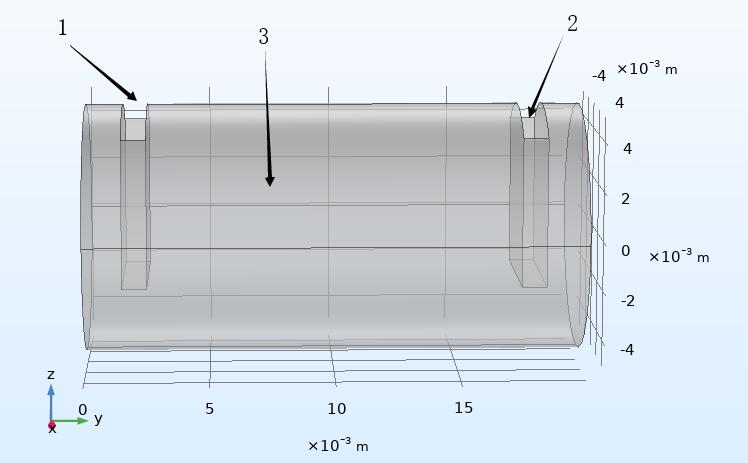
\includegraphics[scale=0.6]{container.jpg}\\
    1)阳极(Anode) 2)阴极(Cathode) 3)电解液(Electrolyte)
    \caption{反应容器物理模型}
    \label{fig:container}
\end{figure}

\section{电化学反应仿真}
\subsection{计算流程}
电解质中每一种离子的通量通过式~\ref{equation:Nernst_Planck}中的Nernst-Planck方程计算得到。再加上
式~\ref{eqation:continuity}连续性方程与式~\ref{equation:neutrality}电中性条件的约束。可以得到离子的
运动情况。
阳极和阴极边界条件通过式~\ref{equation:Butler_Volmer}Butler-Volmer方程给定。电化学反应的过程为:
\begin{equation}
    \mbox{阳极}\quad \ce{2 Cl- - 2e- -> Cl2(g)}
\end{equation}
\begin{equation}
    \mbox{阴极} \quad \ce{2 H2O + 2 e- -> H2(g) + 2OH- }
\end{equation}

根据以上理论我们在COMSOL Multiphysics中进行如下操作:

1)在COMSOL Multiphysics中新建一个一个项目,选择三维模型,添加电化学物理场,
选择考虑电解质迁移影响的“三次分布”电流模型。

2)在几何选项中添加我们上一步完成的物理模型,并定义正负极板电势,以及极板处所发生的的化学反应的方程式与
平衡电位\footnote{使用标准电极电位值},电极动力选表达式选择Butler-Volmer方程。

3)定义溶液中各物质的浓度、电荷数、扩散系数以及溶液电导率等参数。

4)选择细化网格,调整瞬态求解器的时间范围与时间步,开始计算,得到仿真结果。

\subsection{结果与讨论}
图~\ref{fig:cOH1}显示了运行一段时间后,反应容器内$\ce{OH-}$离子的浓度等值面变化。
可以看到阴极处反应产生了大量的$\ce{OH-}$离子,
并在电场力与浓度梯度力的作用下,向溶液体系中扩散。
\begin{figure}[ht]
    \centering
    \subcaptionbox{运行5$s$时$c_{\ce{OH-}}$等值面}% 
                    [6.4cm]{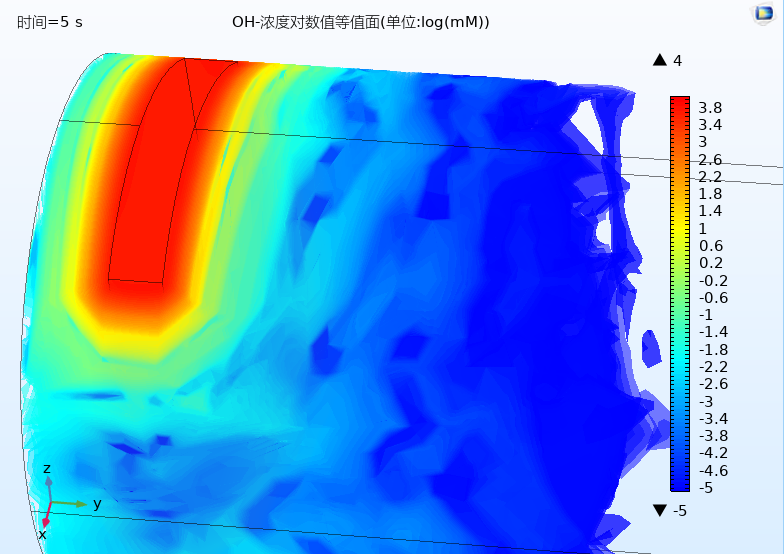
\includegraphics[height=5cm]{cOH等势面5s.png}}
    \hspace{1cm}
    \subcaptionbox{运行15$s$时$c_{\ce{OH-}}$等值面}%
                    %
                    [6.4cm]{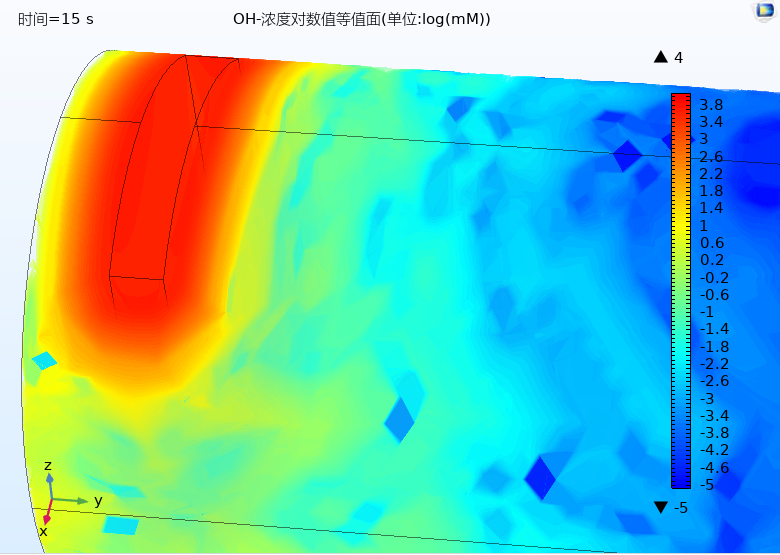
\includegraphics[height=5cm]{cOH等势面15s.png}}
    \centering
    \subcaptionbox{运行30$s$时$c_{\ce{OH-}}$等值面}%
                    %
                    [6.4cm]{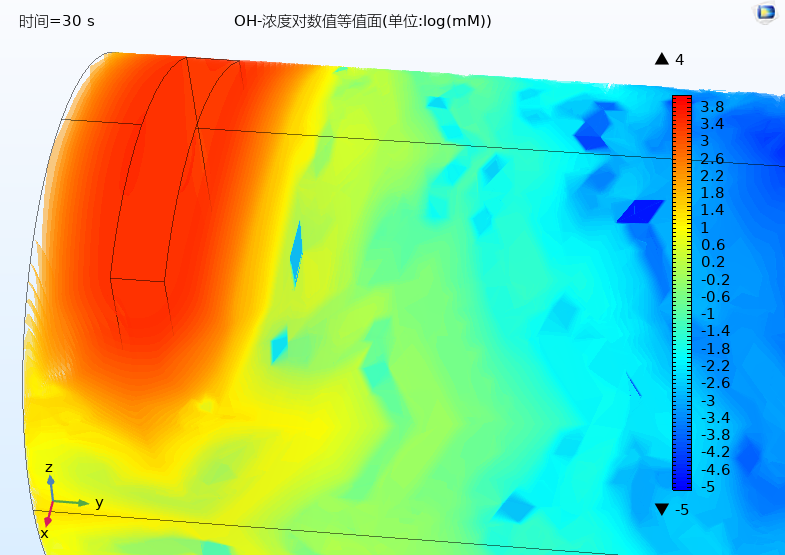
\includegraphics[height=5cm]{cOH等势面30s.png}}
    \hspace{1cm}
    \subcaptionbox{运行50$s$时$c_{\ce{OH-}}$等值面}%
                    %
                    [6.4cm]{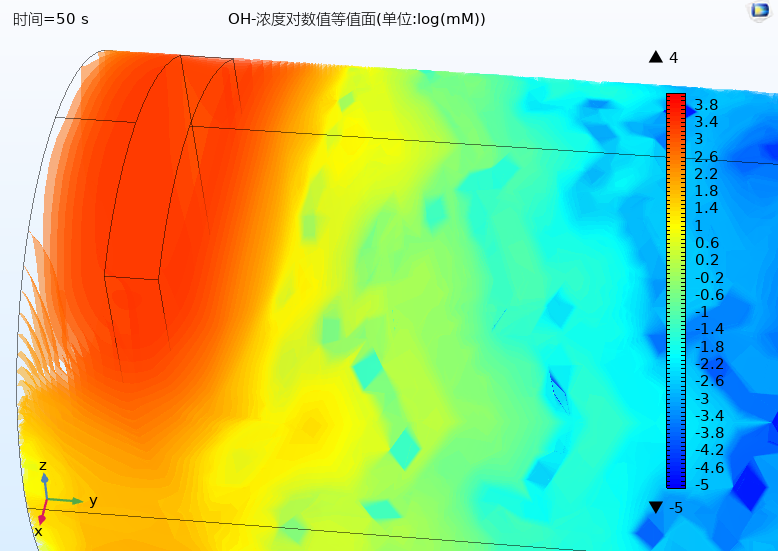
\includegraphics[height=5cm]{cOH等势面50s.png}}
    \caption{$c_{\ce{OH-}}$等值面与运行时间的关系}
    \label{fig:cOH1}
\end{figure}

图~\ref{fig:cOH_distribution}显示,在运行5$s$后,极板上的$c_{\ce{OH-}}$分布基本均匀,
可以近似认为极板上$c_{\ce{OH-}}$处处相等。
\begin{figure}[H]
    \centering
    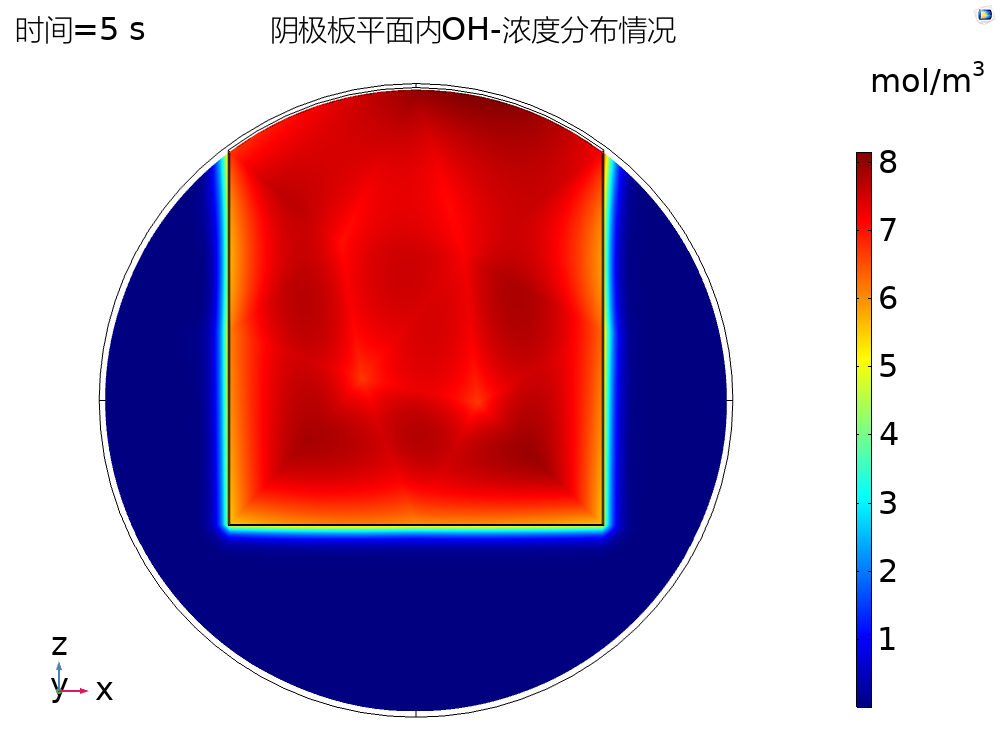
\includegraphics[width=12cm]{cOH分布.png}
    \caption{运行5s时,极板所在平面$c_{\ce{OH-}}$浓度的分布情况}
    \label{fig:cOH_distribution}
\end{figure}

如图~\ref{fig:cOH_t}所示,在运行的前10$s$,由于电信号的激励,电化学反应不断发生,
阴极表面的$c_{\ce{OH-}}$迅速增加,但由于电荷堆积,行程双电层,抑制反应发生,所以
$c_{\ce{OH-}}$的增长速度在变慢。
运行10$s$后,施加的电势被去除,电化学反应停止,溶液中的${\ce{OH-}}$离子主要做自由扩散,
浓度逐渐降低,浓度曲线近似指数函数。
\begin{figure}[H]
    \centering
    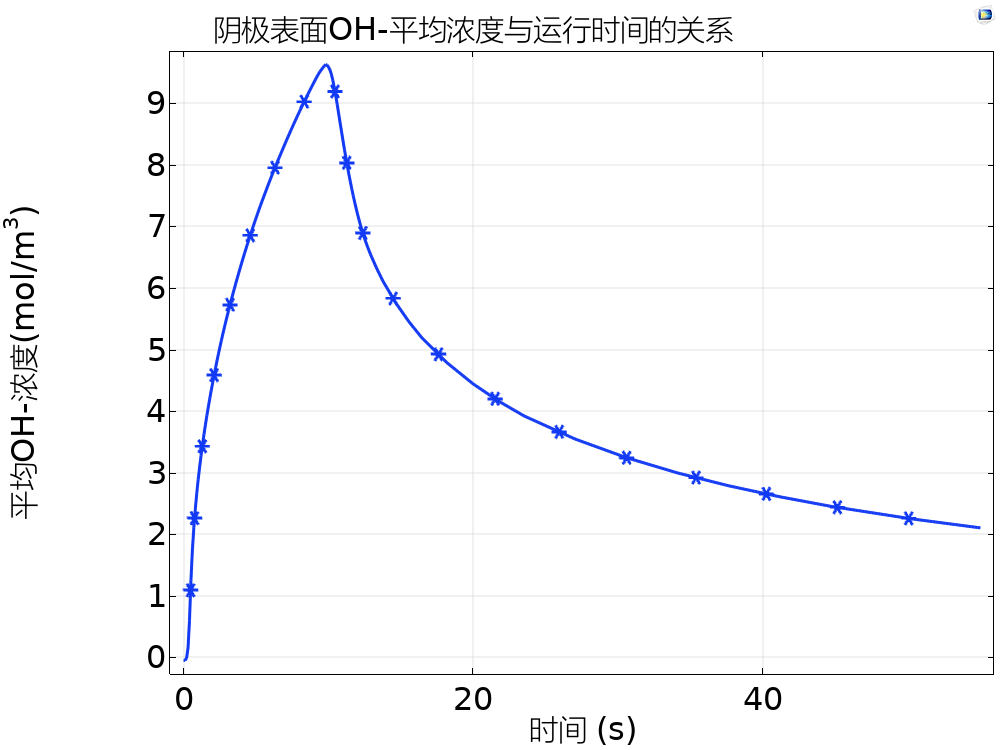
\includegraphics[width=12cm]{cOH曲线.png}
    \caption{极板表面平均$c_{\ce{OH-}}$浓度与时间的关系}
    \label{fig:cOH_t}
\end{figure}

\section{Zr$^{4+}$水解反应仿真}
\subsection{计算流程}
根据式~\ref{rate_equation} 化学反应速率方程,我们知道化学反应速率与反应速率常数$k$以及反应物浓度有关。

松井光二教授与大貝理治教授长期从事金属氧化物的研究,这里我们引用\parencite{40005382310,doi:10.1111/j.1151-2916.2002.tb00131.x}
中,对于$\ce{Zr^4+}$水解时
反应速率常数的研究数据,通过插值法获得我们实验条件下的反应速率常数$k$。计算步骤如下:

1)将电化学反应中,极板表面平均$c_{\ce{OH-}}$浓度与时间的关系的数据导出至txt文档中,采样周期为10$ms$。

2)由于生成的$\ce{OH-}$离子的数量级
远高于固定的$\ce{Zr^4+}$离子,所以我们假设在反应过程中$\ce{Zr^4+}$消耗不会引起$\ce{OH-}$浓度的变化,故$\ce{OH-}$的浓度数据
可以直接代入上一步仿真得到的极板表面平均$c_{\ce{OH-}}$浓度与时间的关系曲线。
在MATLAB中调用浓度时间序列的数据,以10$ms$为采样周期,离散的计算$\ce{Zr^4+}$的消耗曲线。即根据此时$\ce{OH-}$的浓度,计算出
水解反应的速率$v$,然后假定在10$ms$周期内速率为常数,计算这10$ms$内消耗的$\ce{Zr^4+}$。

3)将每一个10$ms$周期内消耗的$\ce{Zr^4+}$的量做累加,得到$\ce{Zr^4+}$的消耗曲线。
%代码见附录
\subsection{结果与讨论}

图~\ref{1stZr}显示了,在第一次激励过程中($0<t<60s$),$\ce{Zr^4+}$随时间而变化的消耗曲线。随着电极表面的$\ce{OH-}$浓度增加,
反应速率将增加,10$s$后,电化学反应停止,电极表面的$\ce{OH-}$浓度因为自由扩散而降低,水解速率也降低。最终可以得到在第一个60$s$的
反应过程中,总共消耗了约2.15层$\ce{Zr^4+}$。
\begin{figure}[H]
    \centering
    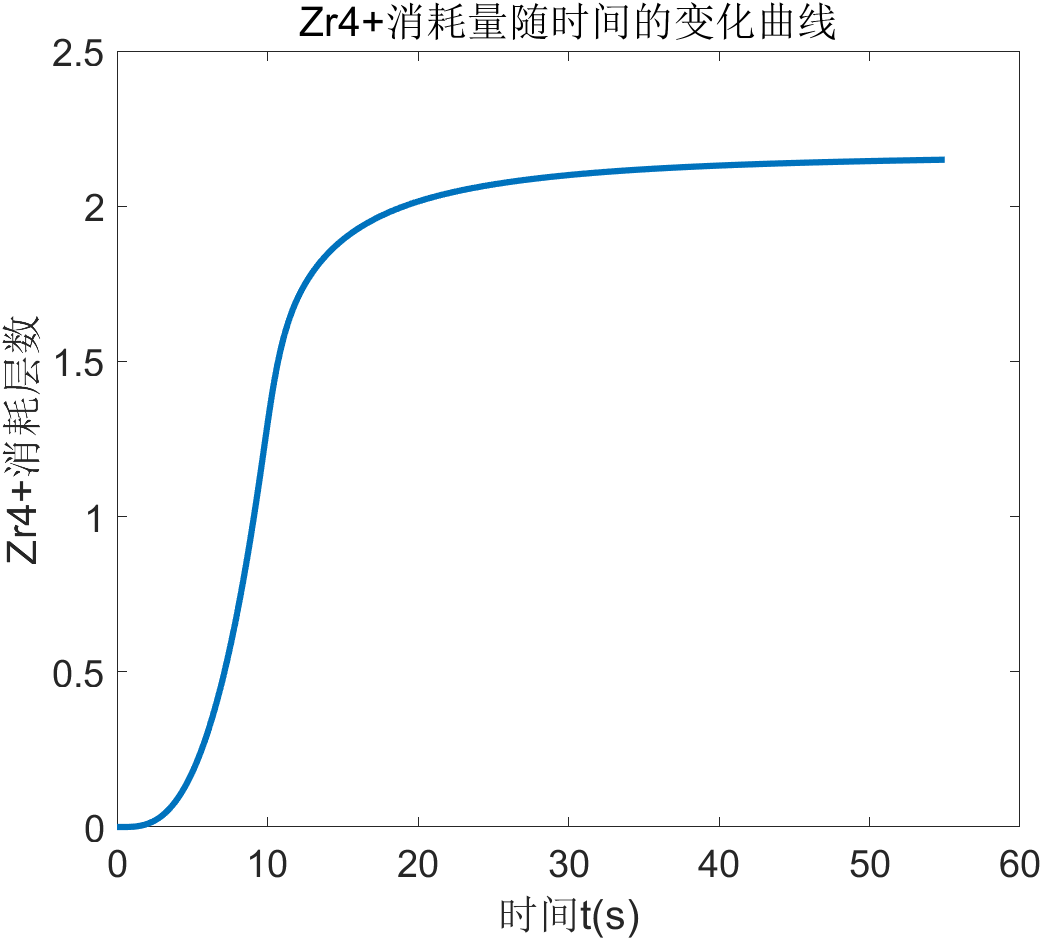
\includegraphics[width=10cm]{Zr4+消耗曲线.png}
    \caption{第一次激励过程中$\ce{Zr^4+}$的消耗曲线}
    \label{1stZr}
\end{figure}

改变反应时间,代入该时间段内的$\ce{OH-}$浓度与$\ce{Zr^4+}$浓度数据,重复上述操作,可以得到激励次数与本次激励内$\ce{Zr^4+}$的消耗量
的序列,如图~\ref{Zrseq}所示。随着反应的进行,$\ce{ZrO2}$溶解的逆反应强度会加剧,$\ce{Zr^4+}$的消耗会导致其浓度降低,最终水解速率会
越来越慢,直至反应达到平衡。在课题组实验中,经过5次电压激励后,DNA的浓度基本不再发生改变,这与仿真结果中$\ce{Zr^4+}$的消耗曲线相吻合。
\begin{figure}[H]
    \centering
    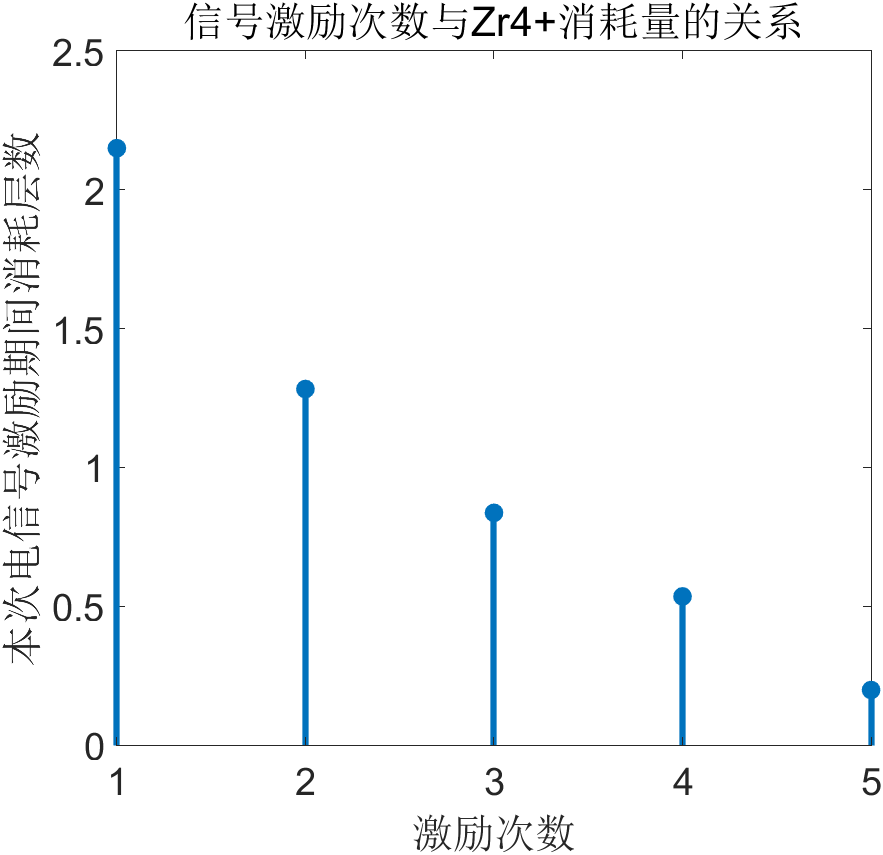
\includegraphics[height=6cm]{每次激励消耗.png}
    \caption{第一次激励过程中$\ce{Zr^4+}$的消耗曲线}
    \label{Zrseq}
\end{figure}

\section{DNA扩散过程仿真}
\subsection{计算流程}
根据式~\ref{equation:Nernst_Planck} Nernst Planck普朗克方程,可以计算出了流体介质中带电化学物质的运动情况。实验所用的DNA为碱基长度
在$20$~$100$左右的单链DNA(ssDNA),在\parencite{Stellwagen2003}一文中可以得到,
在这一长度的DNA分子的扩散系数大约是$D_i=1.52\cdot 10^6cm^2 s^{-1}$。根据~\ref{Nernst-Einstein} Nernst Einstein关系,可以得到
扩散系数$D_i$与扩散迁移率$m_{i,abs}$的关系。再加上式~\ref{eqation:continuity}连续性方程与式~\ref{equation:neutrality}电中性条件的约束。
可以得到DNA分子在电场力与浓度梯度力作用下的运动情况。主要操作如下:

1)在COMSOL Multiphysics中加入“电泳输送”物理场。输入溶液电导率,电泳物质扩散系数等参数。

2)我们将正极的电压改为实验中施加的周期信号。阴极板处,我们放置一个ssDNA的源,将MATLAB中计算得到的DNA释放速度曲线作为流入源的通量曲线代入。

3)配置网格以及求解器等参数,进行仿真运算。

\subsection{结果与讨论}
图~\ref{fig:cDNA1}显示了DNA浓度等值面与运行时间的关系。在第1$s$、6$s$与12$s$,DNA不断被释放出来,可以看到极板的正面浓度不断增加,
并且在电场力的作用下,DNA迅速的向正极迁移。25$s$与50$s$这两张图显示的是,在去除电势之后,$\ce{OH-}$浓度恢复到一个较低的水平,
不再释放新的DNA到溶液中,此时DNA主要做自由扩散运动,浓度梯度越小时,扩散速度越慢。第65$s$显示的是,在第二次施加电势之后,新的DNA
被释放到溶液环境中,重复上述过程。

\begin{figure}[p]
    \centering
    \subcaptionbox{运行1$s$时DNA浓度等值面}% 
                    [6.4cm]{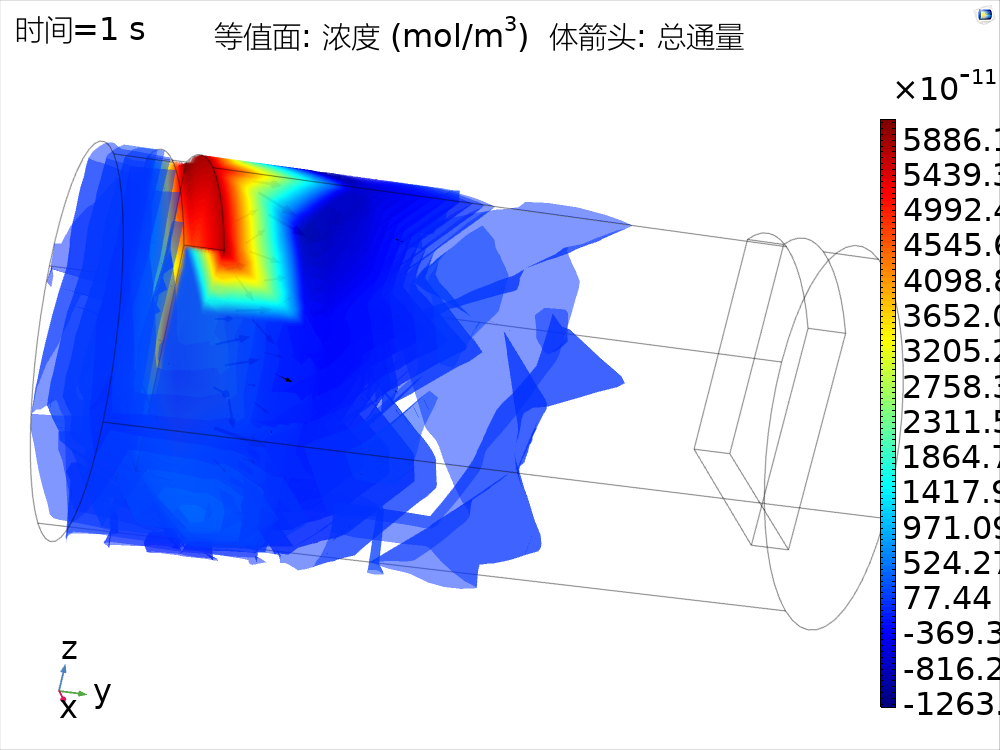
\includegraphics[width=7cm]{cDNA1s.png}}
    \hspace{1cm}
    \subcaptionbox{运行6$s$时DNA浓度等值面}%
                    %
                    [6.4cm]{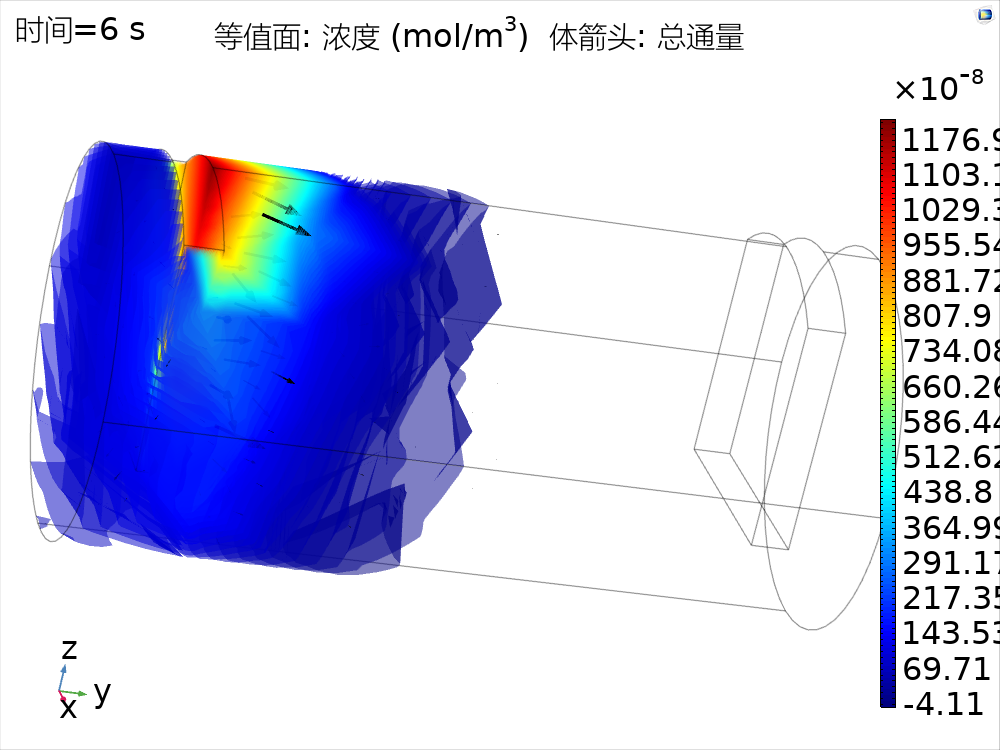
\includegraphics[width=7cm]{cDNA6s.png}}
    \centering
    \subcaptionbox{运行12$s$时DNA浓度等值面}%
                    %
                    [6.4cm]{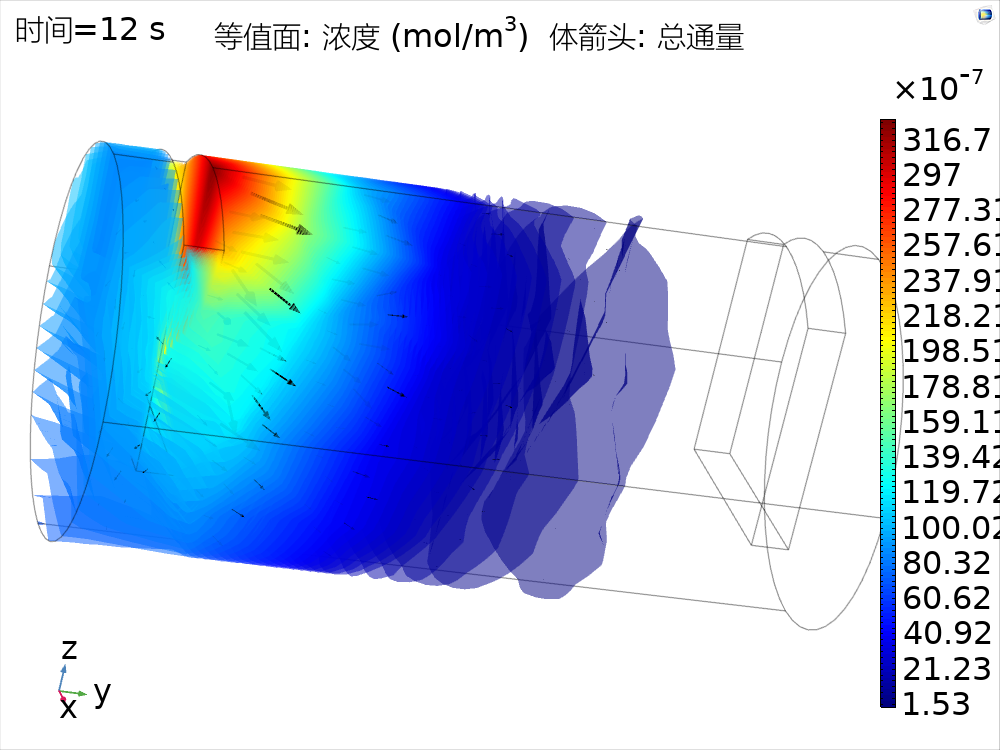
\includegraphics[width=7cm]{cDNA12s.png}}
    \hspace{1cm}
    \subcaptionbox{运行25$s$时DNA浓度等值面}%
                    %
                    [6.4cm]{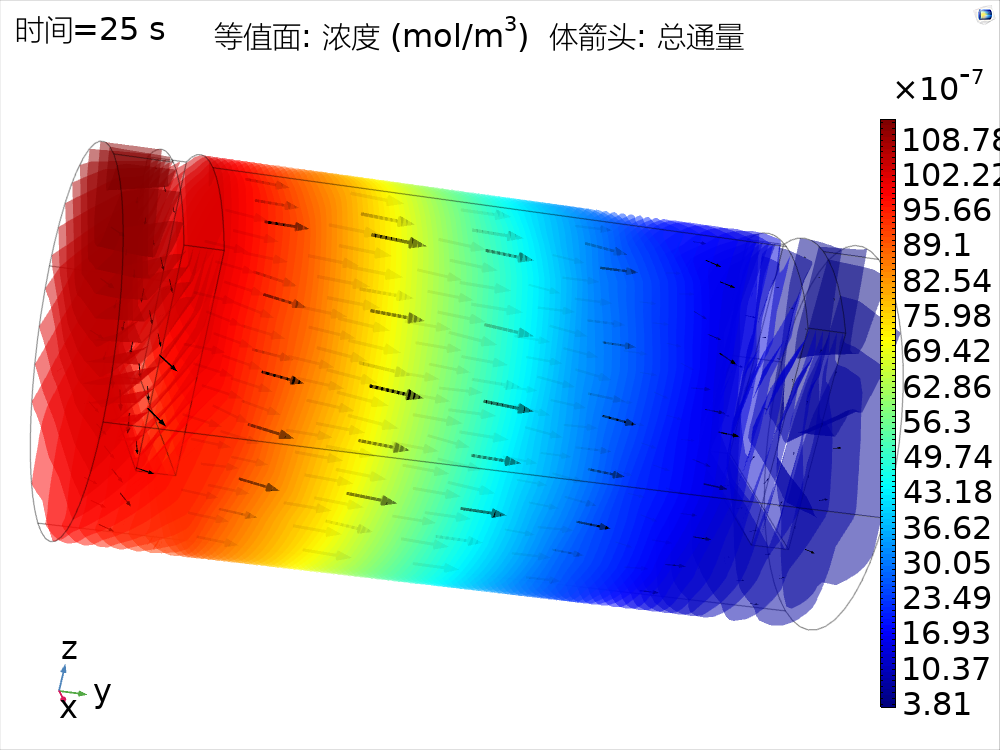
\includegraphics[width=7cm]{cDNA25s.png}}
    \centering
    \subcaptionbox{运行50$s$时DNA浓度等值面}%
                    %
                    [6.4cm]{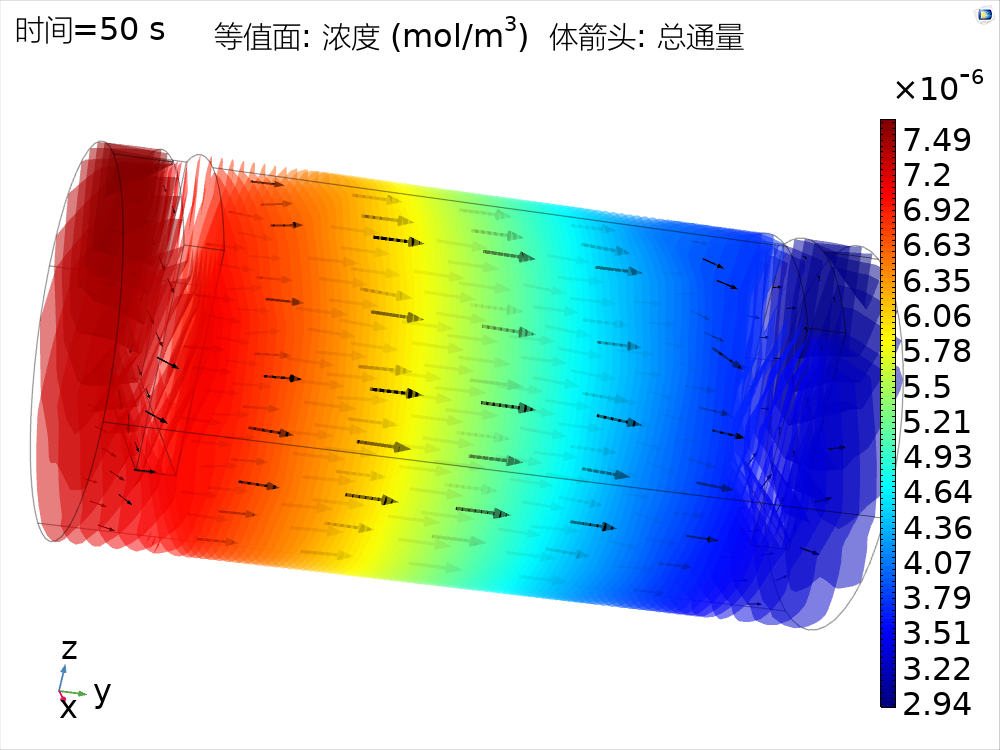
\includegraphics[width=7cm]{cDNA50s.png}}
    \hspace{1cm}
    \subcaptionbox{运行65$s$时DNA浓度等值面}%
                    %
                    [6.4cm]{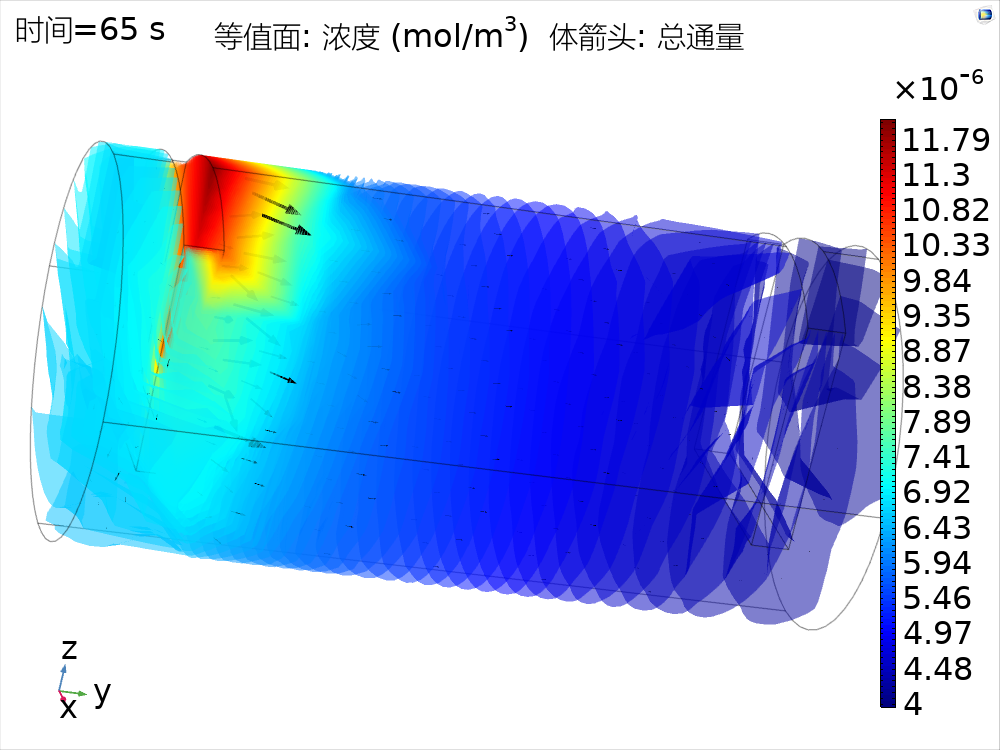
\includegraphics[width=7cm]{cDNA65s.png}}
    \caption{DNA浓度等值面与运行时间的关系}
    \label{fig:cDNA1}
\end{figure}

我们定义阴极一侧的容器底面为$xOy$平面,其圆心为原点,我们在坐标$(0,9mm,0)$处放置一个
浓度探针作为我们的接收机所在的位置,可以看到该探针所在的位置的DNA浓度随时间的变化曲线
如图~\ref{fig:cDNAatP}所示。这个浓度曲线很好的反应了电场力作用与浓度梯度力作用对DNA在
溶液中的运动。
\begin{figure}[H]
    \centering
    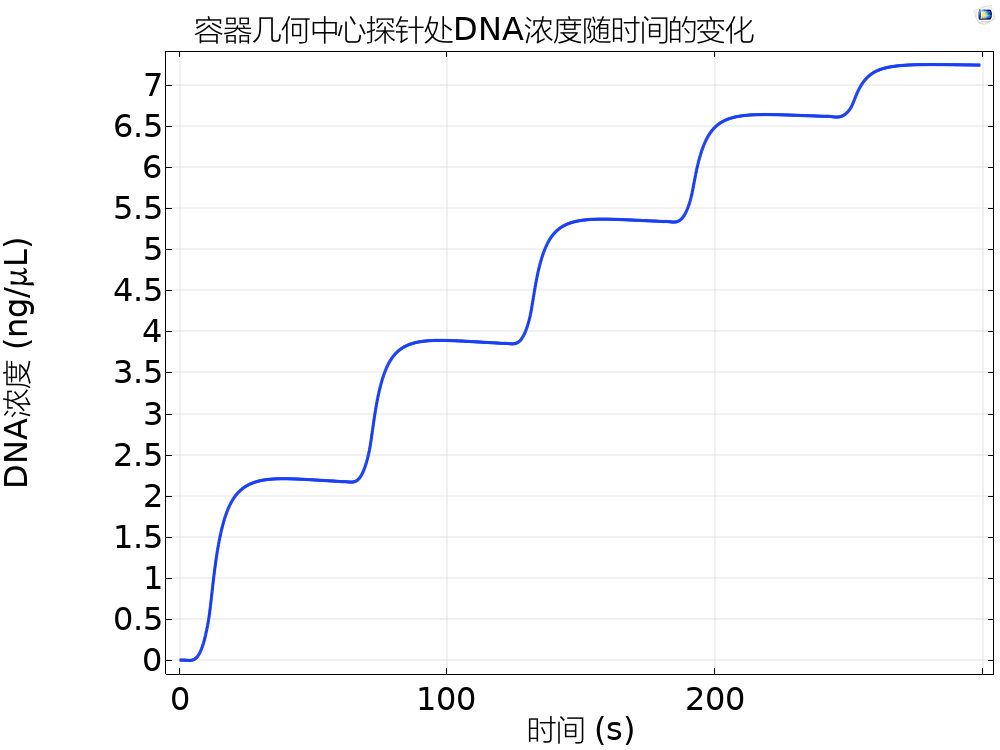
\includegraphics[width=10cm]{cDNA.png}
    \caption{探针处DNA浓度}
    \label{fig:cDNAatP}
\end{figure}

根据式~\ref{fick's 2nd} 菲克第二定律,我们可以求出考虑一维方向上自由扩散的情况下,
距离物质源距离为$x$的位置的该物质浓度曲线$\varphi(x,t)$随时间变化的函数:

\begin{equation}
    \varphi(x,t)= \frac{1}{\sqrt {4 \pi Dt}} exp(-\frac{x^2}{4Dt})
\end{equation}

根据上式,我们假设一种物质$D=0.05m^2\cdot s^{-1}$,在物质源为$x=1m$的位置观测其
浓度随时间变化的曲线,我们称之为信道冲击响应曲线,
简称CIR\footnote{channel impulse response}曲线,
如图~\ref{自由扩散示意图}所示。
\begin{figure}[H]
    \centering
    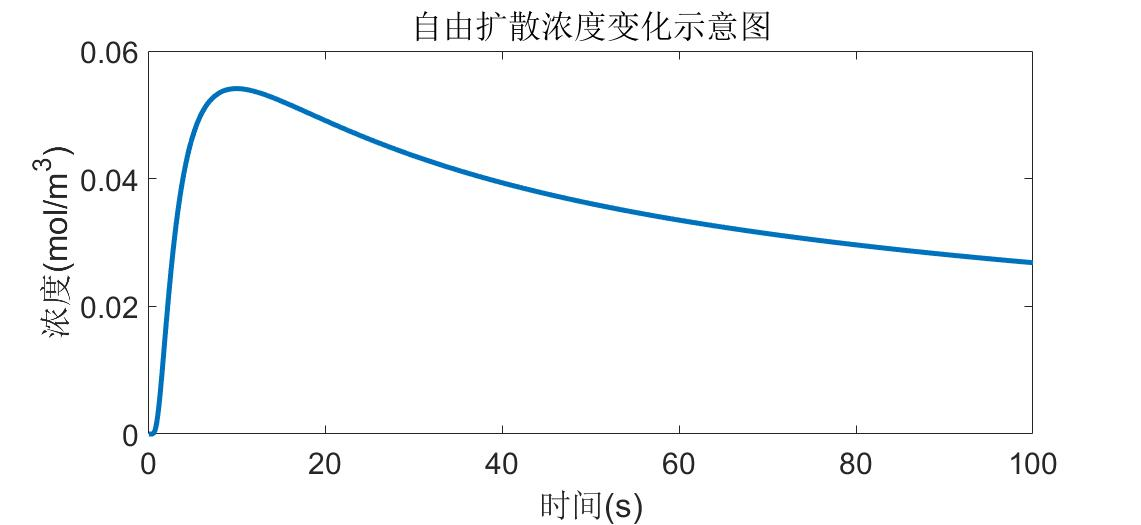
\includegraphics[width=13cm]{自由扩散示意.jpg}
    \caption{自由扩散示意图}
    \label{自由扩散示意图}
\end{figure}

\parencite{8405569}一文中描述了在电场力作用下的CIR曲线,如图~\ref{电迁移}所示,
横轴表示时间,纵轴表示CIR幅度,即被测物质浓度,
红色曲线为电场力作用下的CIR曲线,与之对比的蓝色曲线是自由扩散时的CIR曲线。
\begin{figure}[H]
    \centering
    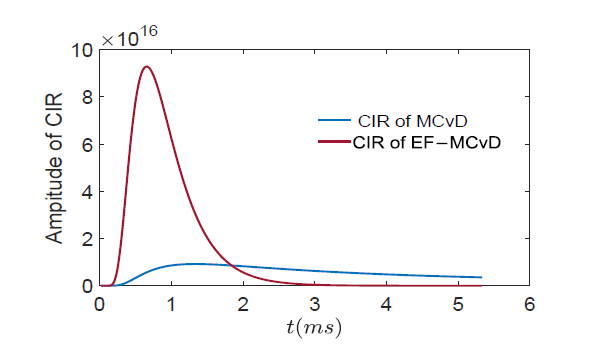
\includegraphics[width=8cm]{电迁移.png}
    \caption{电迁移与自由扩散下浓度变化曲线}
    \label{电迁移}
\end{figure}

将自有扩散与电迁移的效果相叠加后,再与图~\ref{fig:cDNAatP}对比,
可以发现,对DNA扩散过程进行的仿真,很好的还原了DNA分子在电场力与浓度梯度力共同作用下
的扩散情况。将该探针处DNA浓度的变化曲线与课题组所做的实验结果相比照,都表现了DNA浓度该变量会
随释放次数的增加而减少这一现象。

\section{本章小结}
本章介绍了本毕业设计的关键软件COMSOL Multiphysics 在分子通信领域的运用实例。
利用COMSOL Multiphysics 与MATLAB对DNA信息分子分解、释放、传播过程中的电化学反应
、水解反应、电迁移及扩散过程,进行了三维建模与仿真,得到了与先前实验相符的
 DNA 浓度变化曲线数据,很好的还原了DNA分子在电场力与浓度梯度力共同作用下
 的扩散情况,验证了对DNA信息分子发送器建模所获得模型的有效性与正确性。